% fig02_eccentric_construction.tex
% Eccentric anomaly construction: auxiliary circle, ellipse, and affine relations
\documentclass[tikz,border=5pt]{standalone}
\usepackage{amsmath,amssymb}
\usetikzlibrary{angles,quotes,decorations.pathreplacing,calc,positioning,arrows.meta}

\definecolor{accent}{RGB}{0, 100, 170}
\definecolor{highlight}{RGB}{200, 60, 30}
\definecolor{darkgreen}{RGB}{0, 120, 60}
\definecolor{earthblue}{RGB}{40,80,150}
\definecolor{orbitgray}{RGB}{100,100,100}

\begin{document}
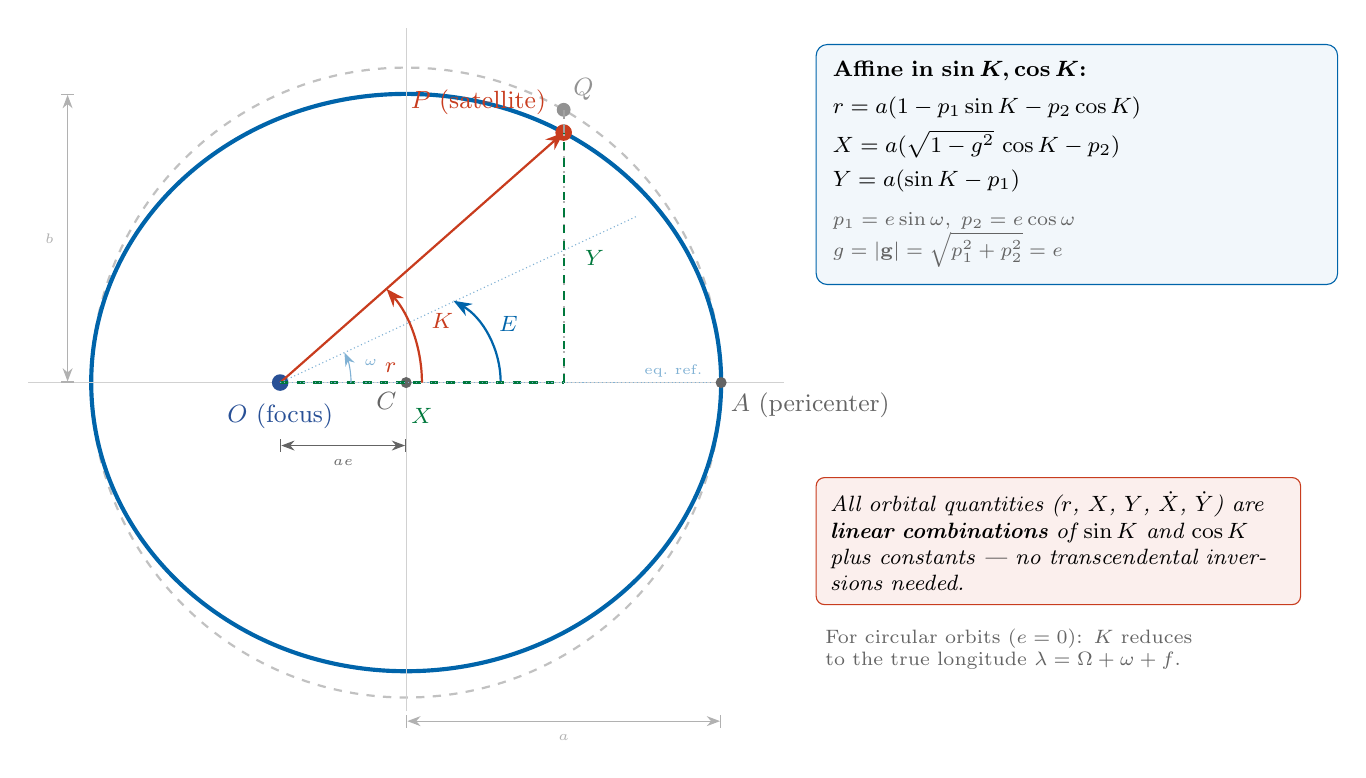
\begin{tikzpicture}[>=Stealth, font=\small]

  % --- Parameters ---
  \pgfmathsetmacro{\smaj}{4.0}        % semi-major axis a
  \pgfmathsetmacro{\ecc}{0.4}         % eccentricity
  \pgfmathsetmacro{\smin}{\smaj*sqrt(1-\ecc*\ecc)}  % semi-minor axis b
  \pgfmathsetmacro{\cfoc}{\smaj*\ecc} % center-to-focus distance ae
  \pgfmathsetmacro{\Edeg}{60}         % eccentric anomaly E in degrees

  % Derived satellite coordinates (relative to center C)
  \pgfmathsetmacro{\Px}{\smaj*cos(\Edeg)}         % x of P rel to C
  \pgfmathsetmacro{\Py}{\smin*sin(\Edeg)}          % y of P rel to C
  % Point Q on auxiliary circle (same x, circle y)
  \pgfmathsetmacro{\Qx}{\smaj*cos(\Edeg)}
  \pgfmathsetmacro{\Qy}{\smaj*sin(\Edeg)}

  % Focus O is at (-ae, 0) relative to center C
  % We place center C at origin, focus O at (-cfoc, 0)
  \pgfmathsetmacro{\Ox}{-\cfoc}

  % X,Y of satellite relative to focus O
  \pgfmathsetmacro{\Xsat}{\Px - \Ox}  % horizontal from focus to P
  \pgfmathsetmacro{\Ysat}{\Py}        % vertical

  % --- Auxiliary circle (dashed, light gray) ---
  \draw[orbitgray!40, dashed, line width=0.8pt] (0,0) circle (\smaj);

  % --- Ellipse (accent, solid) ---
  \draw[accent, line width=1.5pt] (0,0) ellipse ({\smaj} and {\smin});

  % --- Axes (light) ---
  \draw[orbitgray!30, thin] ({-\smaj-0.8},0) -- ({\smaj+0.8},0);
  \draw[orbitgray!30, thin] (0,{-\smin-0.5}) -- (0,{\smaj+0.5});

  % --- Center C ---
  \fill[orbitgray] (0,0) circle (2pt);
  \node[below left, orbitgray] at (0,0) {$C$};

  % --- Focus O (Earth) ---
  \fill[earthblue] (\Ox,0) circle (3pt);
  \node[below, earthblue] at (\Ox,-0.15) {$O$ (focus)};

  % --- Pericenter A ---
  \fill[orbitgray] (\smaj,0) circle (2pt);
  \node[below right, orbitgray] at (\smaj,0) {$A$ (pericenter)};

  % --- Point Q on auxiliary circle ---
  \fill[orbitgray!70] (\Qx,\Qy) circle (2.5pt);
  \node[above right, orbitgray!70] at (\Qx,\Qy) {$Q$};

  % --- Satellite P on ellipse ---
  \fill[highlight] (\Px,\Py) circle (3pt);
  \node[above left, highlight] at ({\Px-0.1},{\Py+0.1}) {$P$ (satellite)};

  % --- Vertical projection line P to Q ---
  \draw[orbitgray!60, densely dashed, line width=0.7pt] (\Px,\Py) -- (\Qx,\Qy);

  % --- Vertical from P down to major axis ---
  \draw[orbitgray!50, dotted, line width=0.7pt] (\Px,0) -- (\Px,\Py);

  % --- Eccentric anomaly arc E from C ---
  \draw[accent, thick, ->] (1.2,0) arc[start angle=0, end angle=\Edeg, radius=1.2];
  \node[accent, font=\footnotesize] at ({1.5*cos(\Edeg/2)},{1.5*sin(\Edeg/2)}) {$E$};

  % --- Radius vector r from focus O to P ---
  \draw[highlight, thick, ->] (\Ox,0) -- (\Px,\Py);
  \node[highlight, midway, above left, font=\footnotesize] at
    ({(\Ox+\Px)/2},{(\Py)/2}) {$r$};

  % --- X coordinate (horizontal from O) ---
  \draw[darkgreen, thick, dashed]
    (\Ox,0) -- (\Px,0);
  \node[darkgreen, below, font=\footnotesize] at ({(\Ox+\Px)/2},-0.2) {$X$};

  % --- Y coordinate (vertical) ---
  \draw[darkgreen, thick, dashed]
    (\Px,0) -- (\Px,\Py);
  \node[darkgreen, right, font=\footnotesize] at ({\Px+0.15},{\Py/2}) {$Y$};

  % --- ae label ---
  \draw[orbitgray, |<->|, thin] (0,-0.8) -- (\Ox,-0.8);
  \node[orbitgray, below, font=\tiny] at ({(\Ox)/2},-0.85) {$ae$};

  % --- a label on auxiliary circle ---
  \draw[orbitgray!50, |<->|, thin] (0,{-\smaj-0.3}) -- (\smaj,{-\smaj-0.3});
  \node[orbitgray!50, below, font=\tiny] at ({\smaj/2},{-\smaj-0.35}) {$a$};

  % --- b label ---
  \draw[orbitgray!50, |<->|, thin] ({-\smaj-0.3},0) -- ({-\smaj-0.3},\smin);
  \node[orbitgray!50, left, font=\tiny] at ({-\smaj-0.35},{\smin/2}) {$b$};

  % --- K angle annotation ---
  % K = E + omega; show it as a wider arc from equinoctial reference
  \pgfmathsetmacro{\omegaAngle}{25}  % argument of pericenter for illustration
  \pgfmathsetmacro{\Kangle}{\Edeg + \omegaAngle}

  % Equinoctial reference direction (dashed line from O)
  \draw[accent!50, densely dotted, thin] (\Ox,0) -- ++({\smaj+1.5},0);
  \draw[accent!50, densely dotted, thin] (\Ox,0) -- ++({(\smaj+1)*cos(\omegaAngle)},{(\smaj+1)*sin(\omegaAngle)});
  \node[accent!50, font=\tiny, right] at ({\Ox+\smaj+0.5},0.15) {eq.\ ref.};

  % omega arc
  \draw[accent!50, thin, ->] ({\Ox+0.9},0) arc[start angle=0, end angle=\omegaAngle, radius=0.9];
  \node[accent!50, font=\tiny] at ({\Ox+1.15},0.25) {$\omega$};

  % K arc from equinoctial reference to the satellite direction
  \pgfmathsetmacro{\satAngle}{atan2(\Py, \Px - \Ox)}
  \draw[highlight, thick, ->] ({\Ox+1.8},0) arc[start angle=0, end angle=\satAngle, radius=1.8];
  \node[highlight, font=\footnotesize] at ({\Ox+2.2*cos(\satAngle/2)},{2.2*sin(\satAngle/2)}) {$K$};

  % --- Formula box (right side) ---
  \node[draw=accent, rounded corners=4pt, fill=accent!5, inner sep=6pt,
        text width=6.2cm, font=\footnotesize, anchor=north west]
    (formulas) at ({\smaj+1.2},{\smaj+0.3}) {%
    \textbf{Affine in $\boldsymbol{\sin K, \cos K}$:}\\[4pt]
    $r = a(1 - p_1 \sin K - p_2 \cos K)$\\[3pt]
    $X = a(\sqrt{1-g^2}\,\cos K - p_2)$\\[3pt]
    $Y = a(\sin K - p_1)$\\[6pt]
    {\color{orbitgray}\scriptsize%
    $p_1 = e\sin\omega,\; p_2 = e\cos\omega$\\
    $g = |\mathbf{g}| = \sqrt{p_1^2 + p_2^2} = e$}
  };

  % --- Callout box ---
  \node[draw=highlight, rounded corners=3pt, fill=highlight!8,
        inner sep=5pt, font=\footnotesize\itshape,
        text width=5.8cm, anchor=north west]
    at ({\smaj+1.2},{-1.2}) {%
    All orbital quantities ($r$, $X$, $Y$, $\dot{X}$, $\dot{Y}$)
    are \textbf{linear combinations} of $\sin K$ and $\cos K$
    plus constants --- no transcendental inversions needed.
  };

  % --- Note for circular orbits ---
  \node[anchor=north west, font=\scriptsize, text=orbitgray, text width=5cm]
    at ({\smaj+1.2},{-3.0}) {%
    For circular orbits ($e=0$): $K$ reduces\\
    to the true longitude $\lambda = \Omega + \omega + f$.
  };

\end{tikzpicture}
\end{document}
